\documentclass[12pt,a4paper]{article}

% Packages
\usepackage[utf8]{inputenc}
\usepackage[T1]{fontenc}
\usepackage{geometry}
\usepackage{graphicx}
\usepackage{xcolor}
\usepackage{hyperref}
\usepackage{listings}
\usepackage{fancyhdr}
\usepackage{titlesec}
\usepackage{enumitem}
\usepackage{booktabs}
\usepackage{array}
\usepackage{longtable}

% Page geometry
\geometry{margin=2.5cm}

% Colors
\definecolor{cfbg}{HTML}{1a1a2e}
\definecolor{cfcard}{HTML}{16213e}
\definecolor{cfborder}{HTML}{0f3460}
\definecolor{cfaccent}{HTML}{e94560}
\definecolor{cftext}{HTML}{eaeaea}

% Hyperref setup
\hypersetup{
    colorlinks=true,
    linkcolor=cfaccent,
    urlcolor=cfaccent,
    pdftitle={CF Filter - Codeforces Problem Filter},
    pdfauthor={Mostafa Kamal}
}

% Header and footer
\pagestyle{fancy}
\fancyhf{}
\fancyhead[L]{\textcolor{cfaccent}{CF Filter}}
\fancyhead[R]{\textcolor{cftext}{Project Report}}
\fancyfoot[C]{\thepage}
\renewcommand{\headrulewidth}{0.5pt}
\renewcommand{\footrulewidth}{0.5pt}

% Section formatting
\titleformat{\section}
  {\normalfont\Large\bfseries\color{cfaccent}}{\thesection}{1em}{}
\titleformat{\subsection}
  {\normalfont\large\bfseries\color{cftext}}{\thesubsection}{1em}{}

% Code listings
\lstset{
    basicstyle=\ttfamily\small,
    backgroundcolor=\color{cfbg},
    frame=single,
    rulecolor=\color{cfborder},
    breaklines=true,
    showstringspaces=false
}

\begin{document}

% Title Page
\begin{titlepage}
    \centering
    \vspace*{3cm}
    
    {\Huge\bfseries\textcolor{cfaccent}{CF Filter}}\\[0.5cm]
    {\Large\textcolor{cftext}{Codeforces Problem Filter}}\\[2cm]
    
    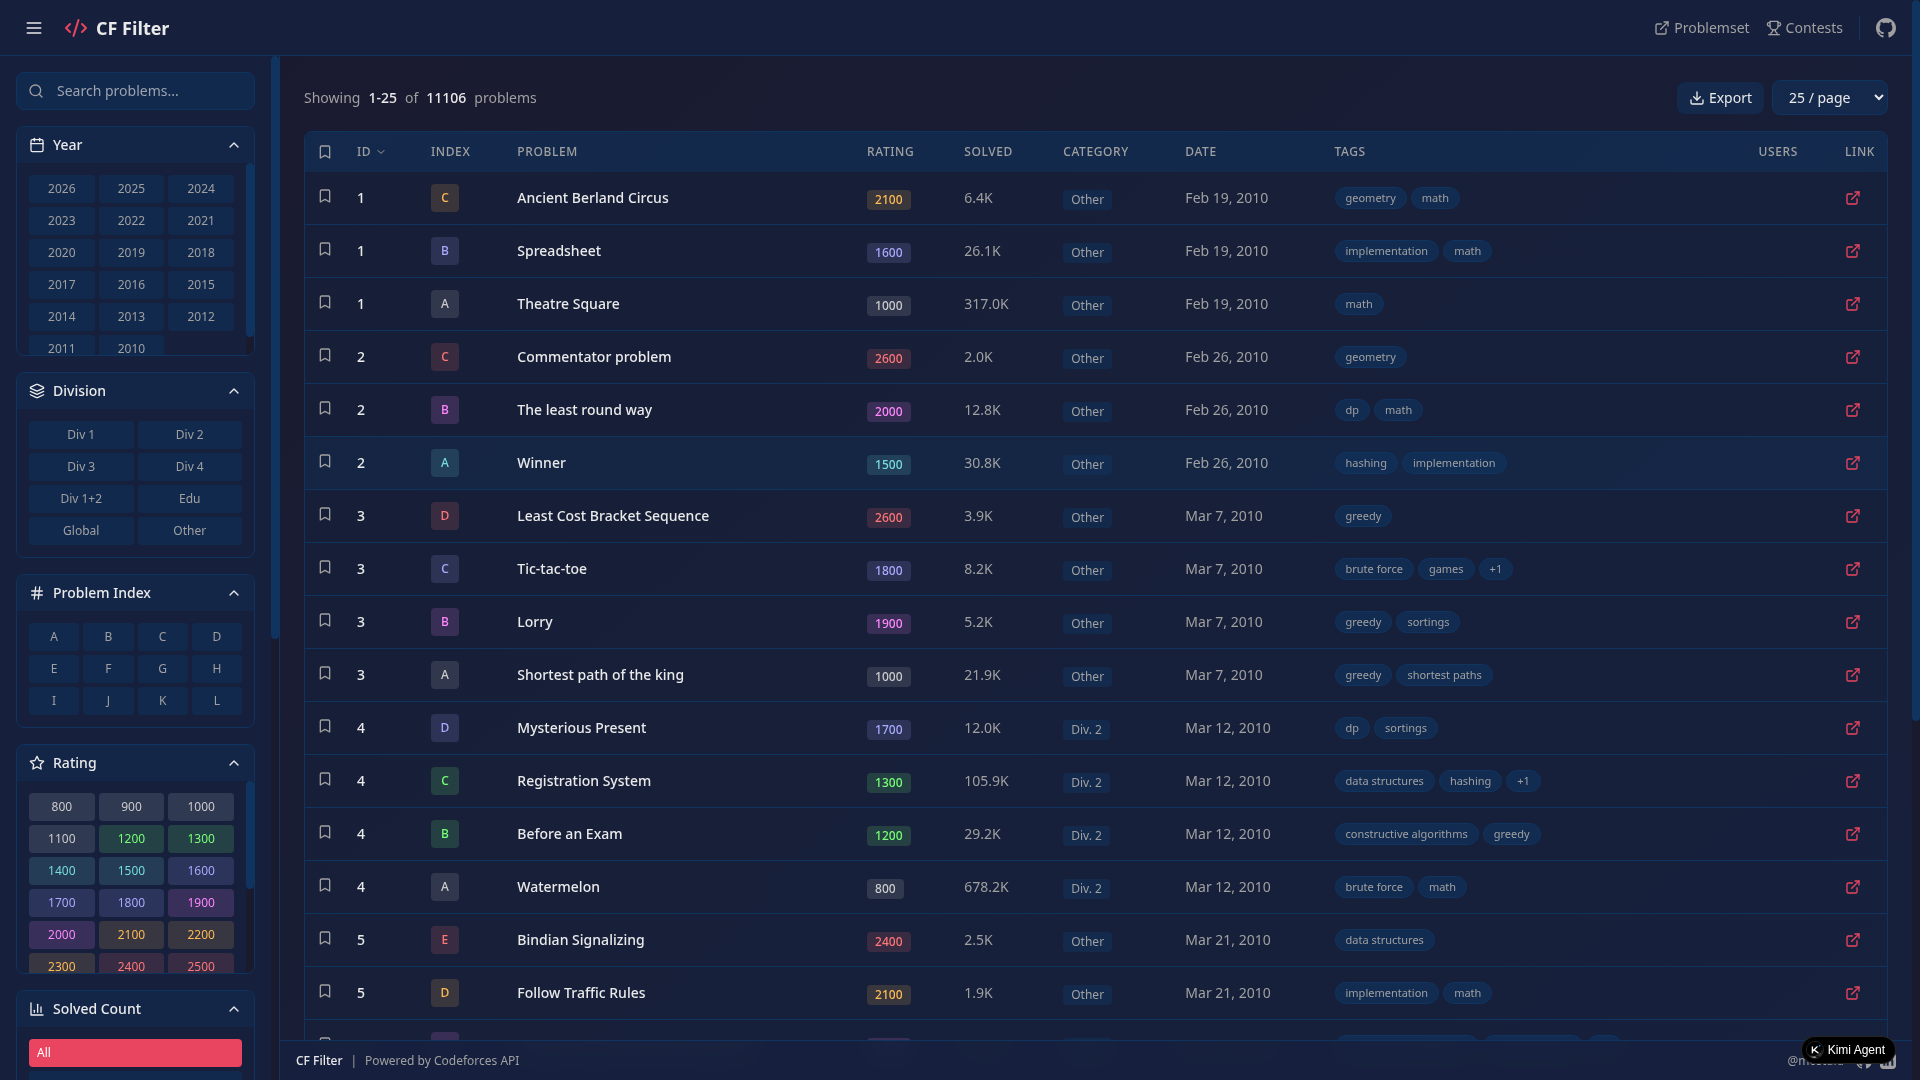
\includegraphics[width=0.8\textwidth]{images/main-dashboard.png}\\[2cm]
    
    {\large\textcolor{cftext}{A Professional Tool for Filtering and Exploring}}\\[0.3cm]
    {\large\textcolor{cftext}{Codeforces Problems}}\\[2cm]
    
    {\large\textcolor{cfaccent}{Version 2.0}}\\[0.5cm]
    {\large\textcolor{cftext}{March 2025}}\\[2cm]
    
    {\large\textcolor{cftext}{Developed by: \textbf{Mostafa Kamal}}}\\[0.3cm]
    {\small\textcolor{cftext}{GitHub: @mostafa-cse}}\\[0.3cm]
    {\small\textcolor{cftext}{Codeforces: @m0stafa}}\\[0.3cm]
    {\small\textcolor{cftext}{LinkedIn: m0stafa-kamal}}
    
    \vfill
\end{titlepage}

% Table of Contents
\tableofcontents
\newpage

% Introduction
\section{Introduction}

\subsection{Overview}
CF Filter is a professional web application designed for competitive programmers to filter, search, and explore Codeforces problems with advanced filtering capabilities. The application provides a clean, responsive interface with a dark theme optimized for extended use.

\subsection{Motivation}
Competitive programmers often need to find specific problems based on various criteria such as:
\begin{itemize}[leftmargin=*]
    \item Problem difficulty (rating)
    \item Contest division (Div 1, Div 2, Div 3, etc.)
    \item Problem tags (DP, Graphs, Math, etc.)
    \item Contest year and date
    \item Solved count (popularity)
    \item Problem index (A, B, C, D, etc.)
\end{itemize}

CF Filter addresses this need by providing a comprehensive filtering system with an intuitive user interface.

\subsection{Target Audience}
\begin{itemize}[leftmargin=*]
    \item Competitive programmers preparing for contests
    \item Students learning algorithms and data structures
    \item Coaches creating problem sets
    \item Anyone interested in exploring Codeforces problems
\end{itemize}

\newpage

% Features
\section{Features}

\subsection{Filter Options}

\subsubsection{Year Filter}
Filter problems by contest year. The application automatically extracts all available years from the Codeforces problemset (2010-2026).

\subsubsection{Division Filter}
Filter problems by contest type:
\begin{itemize}[leftmargin=*]
    \item \textbf{Div 1} - Division 1 contests
    \item \textbf{Div 2} - Division 2 contests
    \item \textbf{Div 3} - Division 3 contests
    \item \textbf{Div 4} - Division 4 contests
    \item \textbf{Div 1+2} - Combined division contests
    \item \textbf{Educational} - Educational Codeforces Round
    \item \textbf{Global} - Global Codeforces Round
    \item \textbf{Other} - Other contest types
\end{itemize}

\subsubsection{Problem Index Filter}
Filter problems by their contest index (A, B, C, D, E, F, G, H, I, J, K, L).

\subsubsection{Rating Filter}
Filter problems by difficulty rating (800-3500). Ratings are color-coded:
\begin{itemize}[leftmargin=*]
    \item \textcolor{gray}{Gray} - $<$ 1200
    \item \textcolor{green}{Green} - 1200-1399
    \item \textcolor{cyan}{Cyan} - 1400-1599
    \item \textcolor{blue}{Blue} - 1600-1899
    \item \textcolor{violet}{Violet} - 1900-2099
    \item \textcolor{orange}{Orange} - 2100-2399
    \item \textcolor{red}{Red} - $\geq$ 2400
\end{itemize}

\subsubsection{Solved Count Filter}
Filter problems by their solved count (popularity):
\begin{itemize}[leftmargin=*]
    \item All
    \item 0 - 500
    \item 500 - 1K
    \item 1K - 5K
    \item 5K - 10K
    \item 10K - 50K
    \item 50K+
\end{itemize}

\subsubsection{Status Filter}
Filter problems based on tracked user submissions:
\begin{itemize}[leftmargin=*]
    \item All - Show all problems
    \item Solved - Show only solved problems
    \item Unsolved - Show only unsolved problems
\end{itemize}

\subsubsection{Tags Filter}
Filter problems by algorithm tags. The application supports all 35+ Codeforces tags including:
\begin{itemize}[leftmargin=*]
    \item 2-sat, binary search, bitmasks, brute force
    \item combinatorics, constructive algorithms, data structures
    \item dfs and similar, divide and conquer, dp, dsu
    \item geometry, graphs, greedy, hashing
    \item implementation, math, number theory
    \item strings, trees, two pointers, and more
\end{itemize}

\subsection{User Tracking}
Track multiple users (up to 7) to see which problems they have solved. Each user is assigned a unique color for easy identification.

\subsection{Problem Display}
Each problem is displayed with:
\begin{itemize}[leftmargin=*]
    \item \textbf{ID} - Contest ID
    \item \textbf{Index} - Problem index (A, B, C, etc.)
    \item \textbf{Problem Name} - Full problem title
    \item \textbf{Rating} - Difficulty rating with color coding
    \item \textbf{Solved Count} - Number of users who solved the problem
    \item \textbf{Category} - Contest division type
    \item \textbf{Date} - Contest date
    \item \textbf{Tags} - Associated algorithm tags
    \item \textbf{Users} - Tracked users who solved the problem
    \item \textbf{Link} - Direct link to Codeforces problem
\end{itemize}

\subsection{Additional Features}

\subsubsection{Search}
Search problems by name, ID, or contest ID.

\subsubsection{Sorting}
Sort problems by ID, rating, solved count, or name in ascending or descending order.

\subsubsection{Pagination}
Navigate through problems with customizable page sizes (5, 10, 15, 20, 25, 30, 50, 100).

\subsubsection{Export to CSV}
Export filtered problems to CSV format for offline analysis.

\subsubsection{Bookmarking}
Bookmark problems for quick access later.

\subsubsection{Filter Persistence}
All filters are automatically saved to localStorage and persist after page refresh.

\newpage

% Technical Implementation
\section{Technical Implementation}

\subsection{Technology Stack}
\begin{itemize}[leftmargin=*]
    \item \textbf{Framework:} Next.js 14 (React 18)
    \item \textbf{Language:} TypeScript
    \item \textbf{Styling:} Tailwind CSS 3.4
    \item \textbf{Icons:} Lucide React
    \item \textbf{HTTP Client:} Axios
    \item \textbf{Deployment:} Static Export
\end{itemize}

\subsection{API Integration}
The application uses the official Codeforces API:
\begin{itemize}[leftmargin=*]
    \item \texttt{problemset.problems} - Fetch all problems and statistics
    \item \texttt{contest.list} - Fetch contest information
    \item \texttt{user.status} - Fetch user submissions
\end{itemize}

\subsection{Data Flow}
\begin{enumerate}[leftmargin=*]
    \item Fetch problems and contest data from Codeforces API
    \item Merge problem data with contest information
    \item Apply user-selected filters
    \item Sort and paginate results
    \item Render filtered problems in the table
\end{enumerate}

\subsection{Responsive Design}
The application is fully responsive with:
\begin{itemize}[leftmargin=*]
    \item Desktop - Full sidebar with all features
    \item Tablet - Collapsible sidebar
    \item Mobile - Optimized table view with hidden columns
\end{itemize}

\newpage

% User Interface
\section{User Interface}

\subsection{Main Dashboard}
The main dashboard provides a comprehensive view of all problems with filtering options in the sidebar.

\begin{figure}[h]
    \centering
    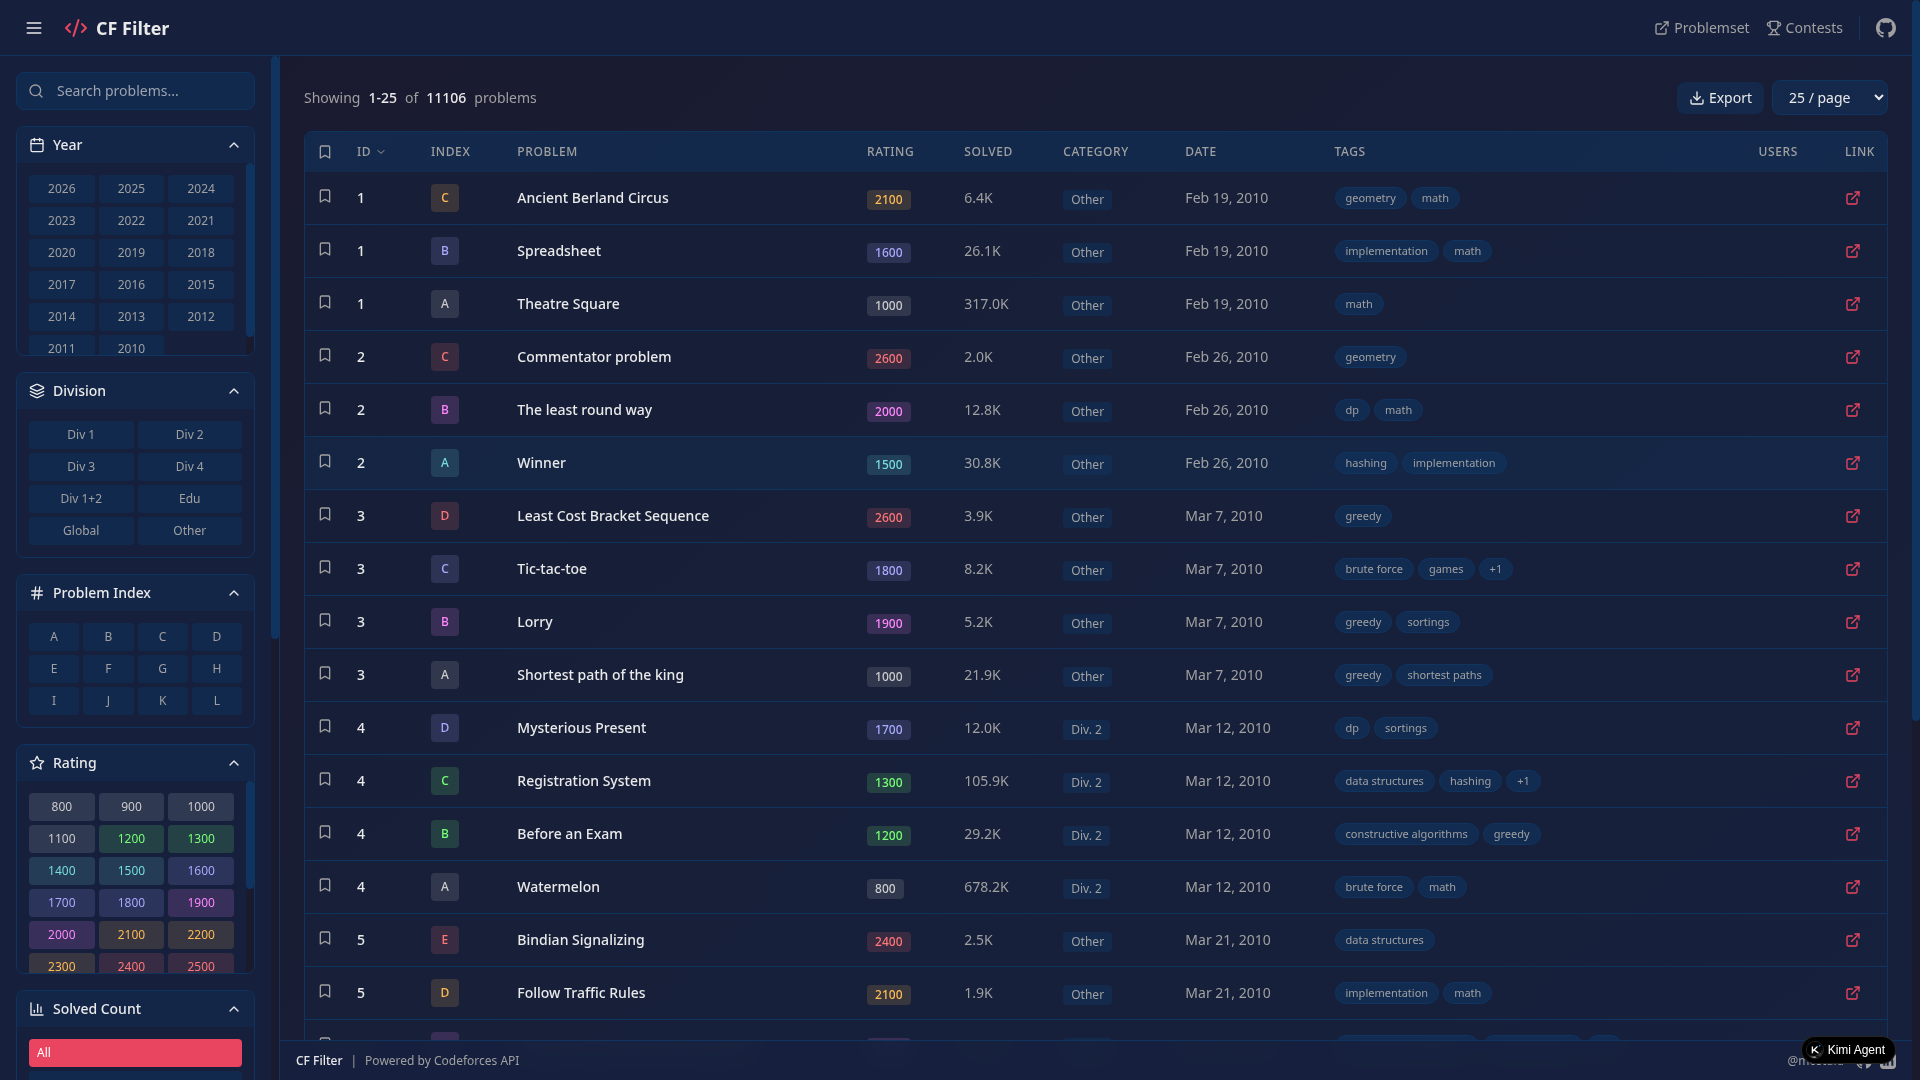
\includegraphics[width=0.95\textwidth]{images/main-dashboard.png}
    \caption{Main Dashboard - Full View with Sidebar}
    \label{fig:main}
\end{figure}

\subsection{Filtered View}
When filters are applied, the problem list updates dynamically to show only matching problems.

\begin{figure}[h]
    \centering
    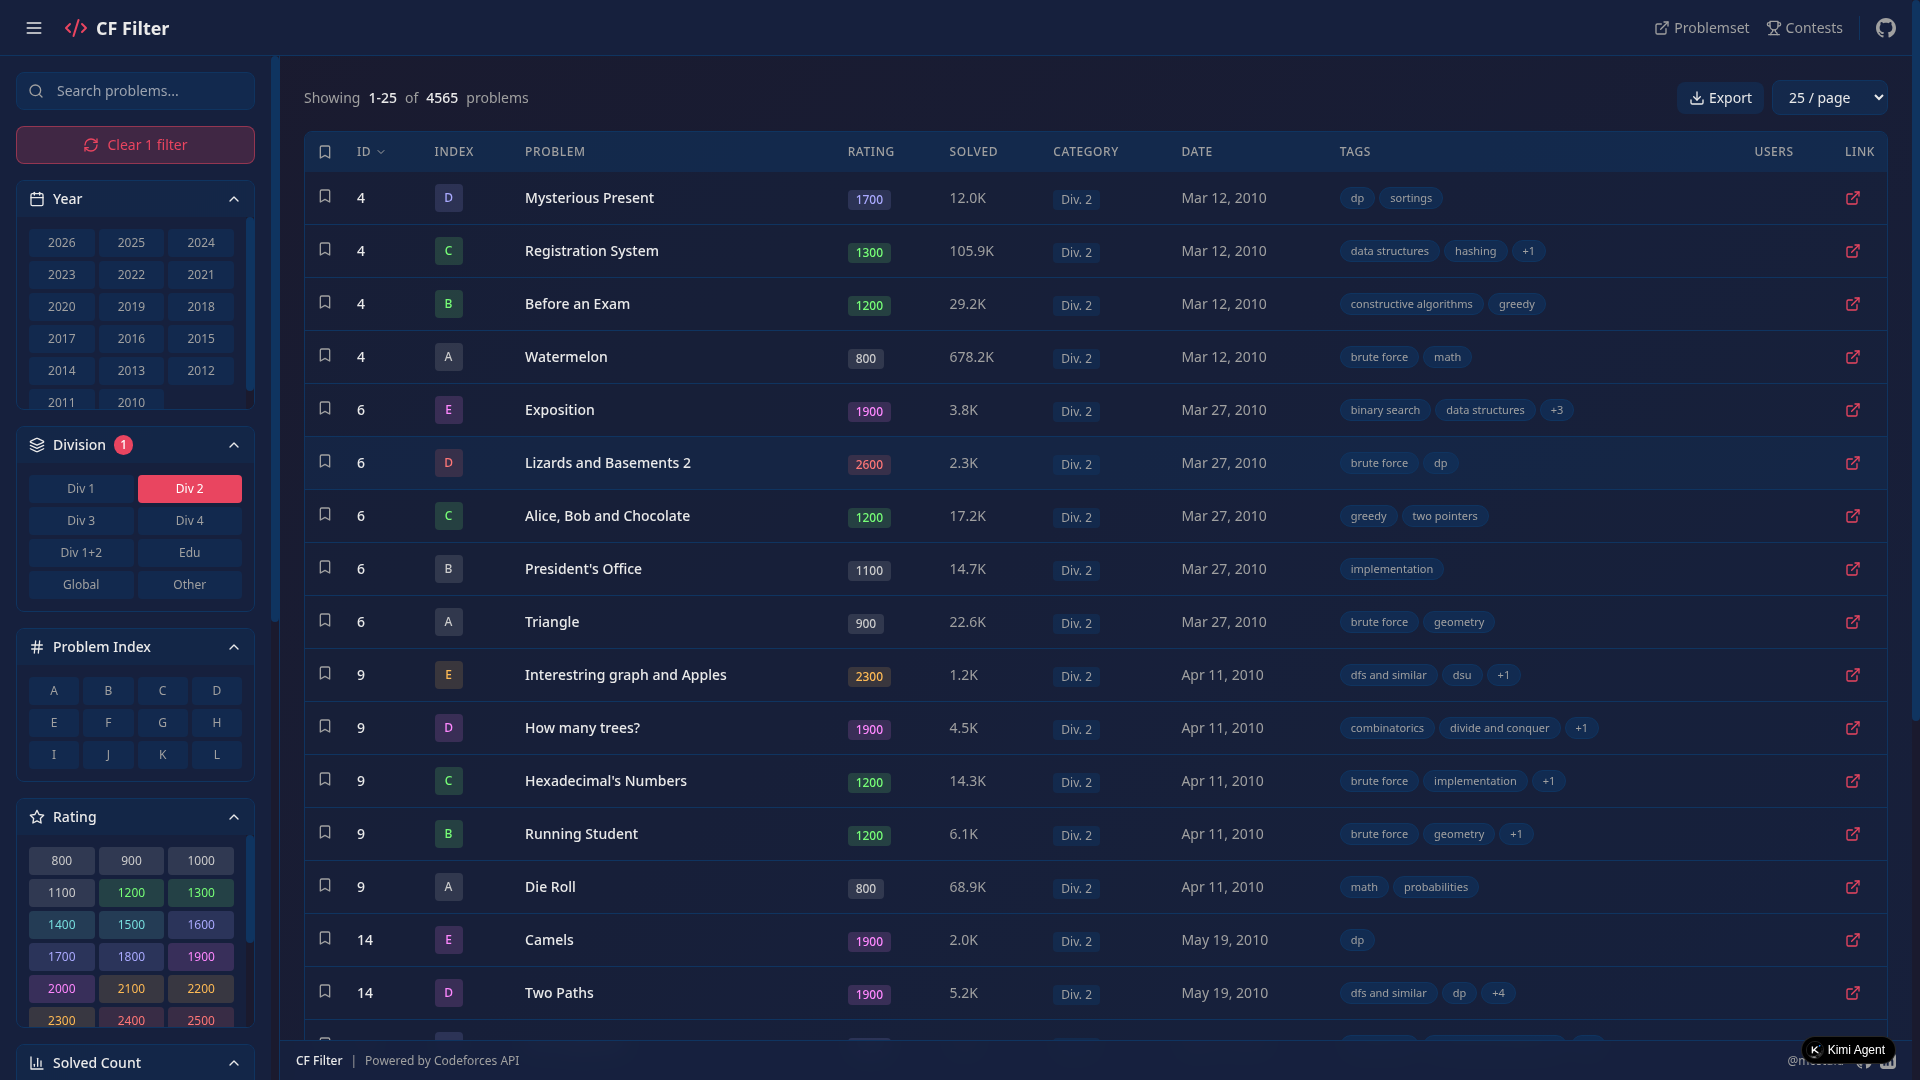
\includegraphics[width=0.95\textwidth]{images/filtered-view.png}
    \caption{Filtered View - Div 2 Problems}
    \label{fig:filtered}
\end{figure}

\subsection{Sidebar Features}
The sidebar contains all filtering options organized into collapsible sections:
\begin{itemize}[leftmargin=*]
    \item Year selection
    \item Division selection
    \item Problem index selection
    \item Rating selection
    \item Solved count range
    \item Status filter
    \item Tags filter with search
    \item User tracking
\end{itemize}

\newpage

% Future Enhancements
\section{Future Enhancements}

\subsection{Planned Features}
\begin{itemize}[leftmargin=*]
    \item \textbf{Problem Recommendations} - Suggest problems based on user history
    \item \textbf{Virtual Contest Mode} - Create virtual contests from filtered problems
    \item \textbf{Problem Notes} - Add personal notes to problems
    \item \textbf{Contest Calendar} - View upcoming contests
    \item \textbf{User Statistics} - Detailed analytics for tracked users
    \item \textbf{Problem Difficulty Graph} - Visual representation of problem distribution
    \item \textbf{Tag Cloud} - Visual tag frequency display
\end{itemize}

\subsection{Performance Improvements}
\begin{itemize}[leftmargin=*]
    \item Implement server-side rendering for faster initial load
    \item Add caching layer for API responses
    \item Implement virtual scrolling for large problem lists
\end{itemize}

\newpage

% Conclusion
\section{Conclusion}

CF Filter provides a professional, feature-rich interface for exploring Codeforces problems. With its comprehensive filtering options, user tracking capabilities, and responsive design, it serves as an essential tool for competitive programmers.

\subsection{Key Achievements}
\begin{itemize}[leftmargin=*]
    \item Successfully implemented all requested filtering options
    \item Fixed Educational, Global, and Other division filters
    \item Added contest date and category display for each problem
    \item Implemented filter persistence using localStorage
    \item Created adjustable and collapsible sidebar
    \item Improved UI/UX with smooth transitions and responsive design
    \item Added bookmarking and export functionality
\end{itemize}

\subsection{Links}
\begin{itemize}[leftmargin=*]
    \item \textbf{Live Website:} \url{https://tv2h3huxbydyy.ok.kimi.link}
    \item \textbf{GitHub:} \url{https://github.com/mostafa-cse}
    \item \textbf{Codeforces Profile:} \url{https://codeforces.com/profile/m0stafa}
    \item \textbf{LinkedIn:} \url{https://www.linkedin.com/in/m0stafa-kamal/}
\end{itemize}

\vfill
\begin{center}
    \textcolor{cfaccent}{\rule{0.5\textwidth}{0.5pt}}\\[0.5cm]
    \textcolor{cftext}{\textbf{CF Filter - Powered by Codeforces API}}\\[0.3cm]
    \textcolor{cftext}{Developed by Mostafa Kamal}\\[0.3cm]
    \textcolor{cftext}{March 2025}
\end{center}

\end{document}
